\documentclass[12pt]{article}

\usepackage[portuguese]{babel}
\usepackage{graphicx}
\usepackage[section]{placeins}
\usepackage{float}
\usepackage{url}
\usepackage{hyperref}

\graphicspath{ {figures} }

\author{João Vitor Maia Neves Cordeiro, Bernardo Schmidt Farias}
\title{Relatório: Instalação e execução do Nanvix}
\date{\today}

\begin{document}

\maketitle

\section{Introdução}

Esse relatório irá descrever os passos utilizados para a execução inicial do \emph{nanvix}, além dos problemas encontrados no caminho e resultado final da instalação.

\section{Instalação e execução}

O processo foi todo realizado em uma máquina hospedeira com o sistema operacional Windows 10, entretanto para facilitar a instalação em relação a compatibilidade de ferramentas foi criada uma instância do WSL (\emph{Windows subsystem for Linux}) em sua versão 2, que oferece acesso ao kernel completo do Linux e outras vantagens. A máquina possui 16GB de RAM, SSD M2 e um processador com 6 núcleos e foi escolhida justamente por ter um hardware mais robusto e moderno, a princípio facilitando o processo de compilação.

\subsection{Clonagem}

O primeiro passo foi a clonagem do repositório, e também foi onde surgiu o primeiro problema, no momento da clonagem foi utilizado o file system do Windows, então todos os arquivos foram criados em NTFS. Isso fez com que o processo de instalação (e build) das ferramentas preliminares fosse muito mais lento, a mesma coisa acontecendo com a build do próprio \emph{nanvix}. Em pesquisa posterior na \href{https://docs.microsoft.com/en-us/windows/wsl/compare-versions}{documentação} do WSL2 descobrimos que a principal desvantagem da versão 2 em comparação com a versão 1 é a queda na performance durante o compartilhamento de arquivos entre os dois file systems. Dessa forma, para uma próxima instalação ficou o aprendizado de clonar o repositório já dentro do WSL2 com o formato de arquivos da máquina virtual.

\subsection{Ferramentas e dependências}

Depois da clonagem, foram instaladas as dependências listadas no relatório (make, toolchain e bochs), apesar de demorarem para executar em virtude dos problemas com o WSL2 (o script setup-toolchain.sh levou pouco mais de uma hora), a instalação das ferramentas foi concluída com sucesso na máquina. 

\subsection{Compilação}

Passando para a compilação do \emph{nanvix}, o primeiro comando make foi executado sem erros, mas durante a execução do segundo comando ele foi interrompido com o o erro que aparece na imagem abaixo. Depois de consultar um colega que trabalha com o \emph{nanvix} descobrimos que faltava uma dependência a ser instalada, o \textbf{mkisofs} que pode ser instalado pelo gerenciador de pacotes do Ubuntu. Com a instalação dessa dependência finalizada, executamos novamente o script \texttt{make image} e ele terminou com sucesso.

\begin{figure}[H]
    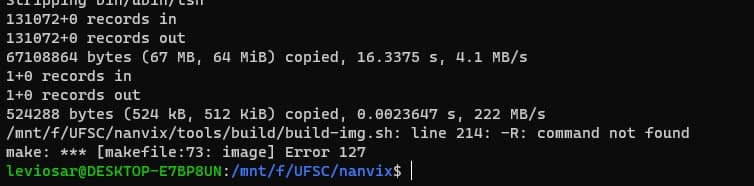
\includegraphics[width=\linewidth]{error.jpg}
    \caption{Erro que ocorreu ao rodar \texttt{make image} sem o \textbf{mkisofs} instalado no sistema.}
\end{figure}

\subsection{Execução}

Por último, realizamos a execução do \emph{nanvix} usando \texttt{bash tools/run/run.sh} e ele abriu sem mais problemas. Observamos também que um processo chamado "Vmmem" começou a utilizar quantidades razoáveis de recursos da máquina, provavelmente o "combo" de rodar WSL2, Bochs e Nanvix consome bastante memória. 

\begin{figure}[H]
    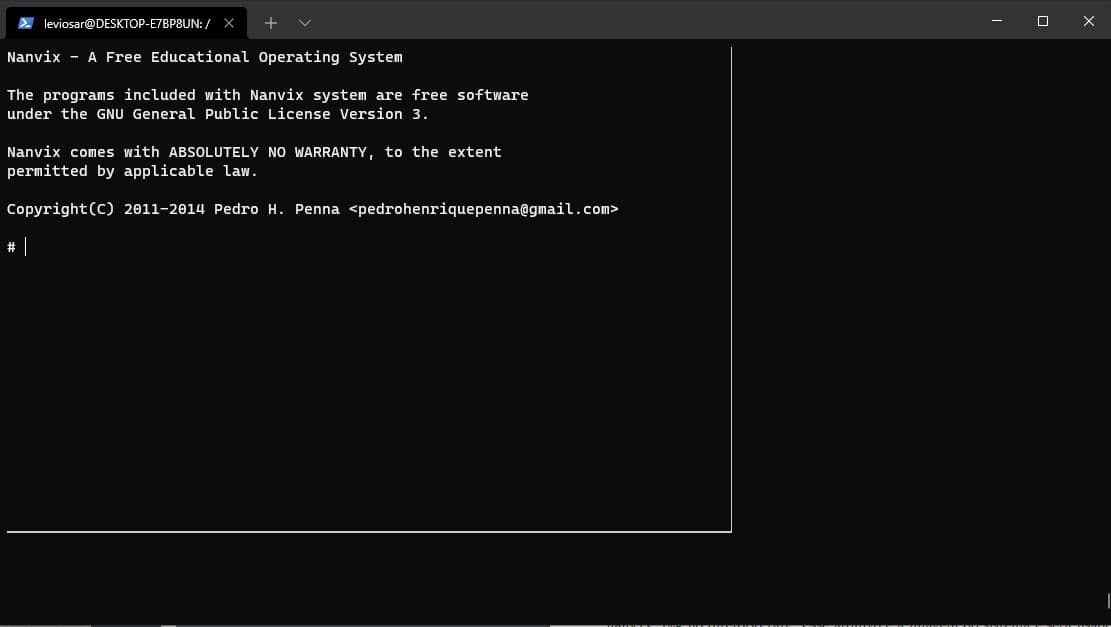
\includegraphics[width=\linewidth]{runnign.jpg}
    \caption{\emph{nanvix} executando.}
\end{figure}

Em conclusão, a instalação e execução do \emph{nanvix} foi relativamente simples, tivemos apenas dois problemas durante a execução do trabalho, um deles causado por nós mesmos ao clonarmos o repositório no file system do Windows, e o segundo a ausência de uma dependência para a criação da imagem do \emph{nanvix}. Fica como sugestão a adição de uma nota ou aviso no tutorial de instalação sobre o \textbf{mkisofs}. 

\end{document}